\documentclass{article}

\usepackage{graphicx}

\begin{document}

\section{Abstract}

K3 is a famous Flemish music group.
Recently they have changed their formation.
Rumors claim that the new formation is worse
than the old one.
Here, we investigate if that claim is true,
based on reviews of their music before
and after the new formation.
We find that the new formation is 
[worse/equal/better].

\section{Introduction}

K3 is a famous Flemish music group
starting in around ?1990.
The band consists out of three girls
and has had three formations, of which
the last one raplaced all three girls,
resulting in a completely new group.

Rumors on internet fora claim that the new
formation is worse. Their music would be
worse. It is unknown if these rumor are true.

In this research, we will test if the new
formation produces music that is as enjoyable
as the old formation.

\section{Hypotheses}

\begin{itemize}
  \item $\mathcal{H}_1$: 
  ratings given to the songs given
  to the previous formation are as high
  as ratings given to the songs given to the
  current formation.
\end{itemize}

\section{Methods}

\paragraph{Data set}
We obtain ratings (which are values from
1 to 10, where 1 is worst and 10 is best) 
from a website in which two people
have rated K3 songs. 

\paragraph{Statistical test}
We do not assume that the 
ratings follows a normal distribution. 
Due to this,
we use a Mann-Whitney U test to test if
the distributions are the same.
We will be using a value of alpha of 0.05,
because there has not been done any previous
research on this.

If the p value if below the alpha value,
the groups are differently enjoyable.
Else, we will conclude the groups 
are equally enjoyability.

\section{Results}

We get a p-value of ? from our
Mann-Whitney U. 

The ratings for the two groups are plotted in
figure 1. 

\begin{figure}[!htbp]
  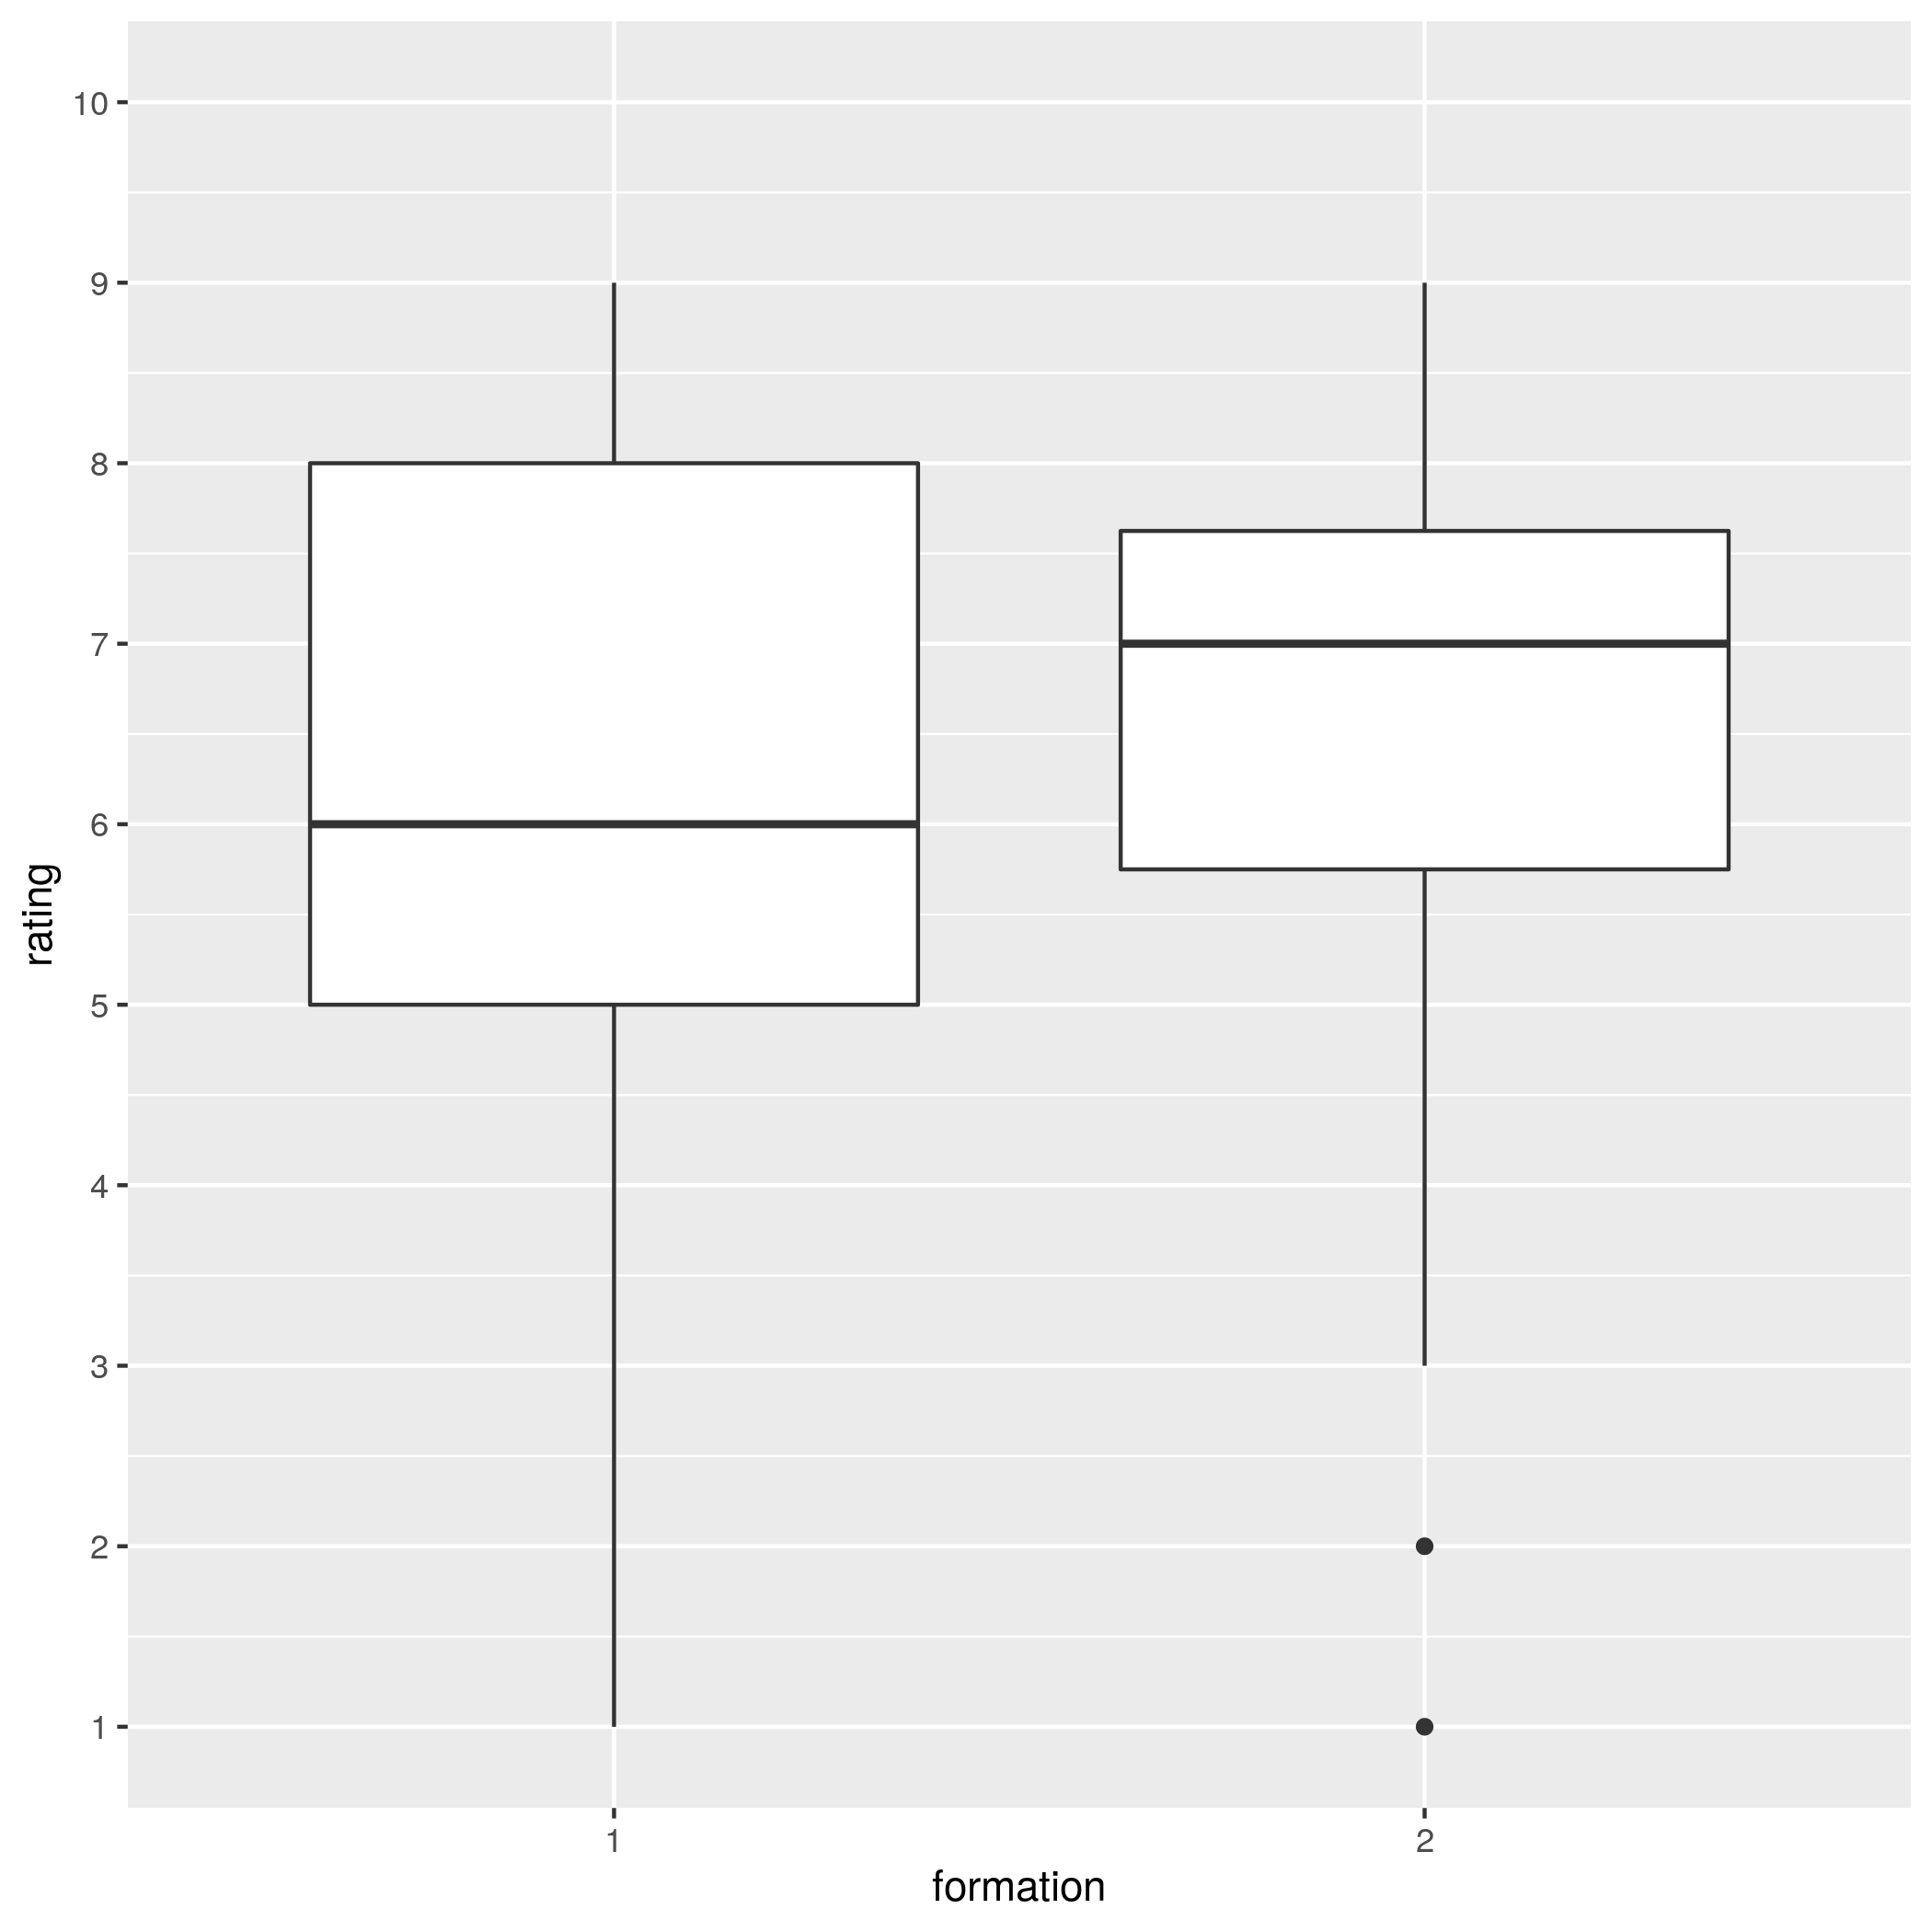
\includegraphics[width=\textwidth]{figure_1.png}
  \caption{
    Ratings for the two formation. 
  }
  \label{fig:1}
\end{figure}

\section{Conclusion}

From our p-value we conclude that
the groups are [equally/differently] enjoyable.

[If there is a difference, then:]
We observe in figure 1 that the [first/second]
group is more enjoyable.

\section{Discussion}

The Mann-Whitney U test cannot calculate
the exact p-value for values that are identical
between the two samples. We expect this is
not a problem.

We obtained the data from the reviews done
by only two people. This may results in
a bias. 
Additionally, only one person reviewed
songs of both formations and not all
songs have been reviewed.
Because it is the only data
set available, there is no other option.

\section{Supplementary materials}

\begin{table}
  \input{stats.latex}
  \caption{
    Stats
  }
  \label{table:stats}
\end{table}

\begin{figure}[!htbp]
  \includegraphics[width=\textwidth]{formations.png}
  \caption{
    Formations
  }
  \label{fig:formations}
\end{figure}


\end{document}
